\section{Evaluation Comparison}\label{sec:result_comparison}

\paragraph{Which Context Enrichment Method performed best in general?}
\begingroup
\renewcommand{\arraystretch}{1.5}
\begin{table}
	\begin{tabularx}{\textwidth}{l c*{3}{Y}}
		\toprule
		Method & Precision & Recall & F-Measure \\
		\midrule
		 Embedded Context & 0.797 & 0.921 & 0.854 \\
		 Neighbouring Nodes & 0.787 & 0.887 & 0.834 \\
		 External Source & 0.729 & 0.899 & 0.805 \\
		 None & 0.674 & 0.910 & 0.775 \\
		\bottomrule
	\end{tabularx}
	\caption{Aggregated results of all datasets~(ranked by F-Measure)}
	\label{table:bench_p_r_f_combined}
\end{table}
\endgroup

\begin{figure}
	 \centering
	 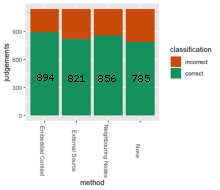
\includegraphics[width=0.75\textwidth]{plots/comparison/barplot_all_judgements}
	 \caption{Combined accuracy of crowdsourcing methods}\label{fig:results_accuracy_combined}
\end{figure}

Lorem ipsum dolor sit amet, consectetur adipisicing elit, sed do eiusmod tempor incididunt ut labore et dolore magna aliqua. Ut enim ad minim veniam, quis nostrud exercitation ullamco laboris nisi ut aliquip ex ea commodo consequat. Duis aute irure dolor in reprehenderit in voluptate velit esse cillum dolore eu fugiat nulla pariatur. Excepteur sint occaecat cupidatat non proident, sunt in culpa qui officia deserunt mollit anim id est laborum.

\paragraph{Did the crowd perform better with context?}
% No chart needed, the charts from the question above can be used %
Lorem ipsum dolor sit amet, consectetur adipisicing elit, sed do eiusmod tempor incididunt ut labore et dolore magna aliqua. Ut enim ad minim veniam, quis nostrud exercitation ullamco laboris nisi ut aliquip ex ea commodo consequat. Duis aute irure dolor in reprehenderit in voluptate velit esse cillum dolore eu fugiat nulla pariatur. Excepteur sint occaecat cupidatat non proident, sunt in culpa qui officia deserunt mollit anim id est laborum.

\paragraph{For which concepts were the crowd wrong?}
% Table show 1st, 2nd and 3rd of overall concepts that were judged incorrectly by the crowd for any dataset. %
% Table layout --> see notes %
Lorem ipsum dolor sit amet, consectetur adipisicing elit, sed do eiusmod tempor incididunt ut labore et dolore magna aliqua. Ut enim ad minim veniam, quis nostrud exercitation ullamco laboris nisi ut aliquip ex ea commodo consequat. Duis aute irure dolor in reprehenderit in voluptate velit esse cillum dolore eu fugiat nulla pariatur. Excepteur sint occaecat cupidatat non proident, sunt in culpa qui officia deserunt mollit anim id est laborum.

\paragraph{Was there a correlation between Inter-rater Agreement and Accuracy}
% Scatterplot of discrete values (http://www.r-graph-gallery.com/5-correlation-of-discrete-variables/) %
% y-axis: Agreement ratio (0.6, 0.8, 1) ; x-axis: Accuracy (0, 1, 2, 3, 4, 5) $
% Merge all datasets and create plot for each method %
Lorem ipsum dolor sit amet, consectetur adipisicing elit, sed do eiusmod tempor incididunt ut labore et dolore magna aliqua. Ut enim ad minim veniam, quis nostrud exercitation ullamco laboris nisi ut aliquip ex ea commodo consequat. Duis aute irure dolor in reprehenderit in voluptate velit esse cillum dolore eu fugiat nulla pariatur. Excepteur sint occaecat cupidatat non proident, sunt in culpa qui officia deserunt mollit anim id est laborum.

\paragraph{What other observations were found?}
% No plots/tables needed, just description %
Lorem ipsum dolor sit amet, consectetur adipisicing elit, sed do eiusmod tempor incididunt ut labore et dolore magna aliqua. Ut enim ad minim veniam, quis nostrud exercitation ullamco laboris nisi ut aliquip ex ea commodo consequat. Duis aute irure dolor in reprehenderit in voluptate velit esse cillum dolore eu fugiat nulla pariatur. Excepteur sint occaecat cupidatat non proident, sunt in culpa qui officia deserunt mollit anim id est laborum.